% 1. novel approach, why? protection goals and performance → security and efficiency
% 2. what precisely was done at the TUD chair → say that their research proved the potential of NC and that's why we persue it here again
% 3. NC provides no confidentiality/integrity guarantees → we implement encryption+authentication
% 3.1 Availability only partially adressed
% 3.2 recall NoC architecture → this is implemented in the network interfaces
% 4. Different variants envisioned (3 methods) + comparison with uncoded variant where applicable
% 5. Multiple paths focus → why multiple paths in the first place? → chance to avoid compromised routers, still have enough flits
%    thanks to NC
% 6. Routing strategies: deterministic vs. non-deterministic routing → XY, smart random XY, ROMM+XY, ROMM+srXY
% 7. Attacker/Threat model
% 8. Evaluation
% Always refer to the chapters that explain this in detail
In this thesis, a novel approach for securing the communications in a \gls{noc}-based \gls{mpsoc} is pursued. The goal is to design and implement a protocol that
remedies both accidental and malicious modifications to the transmitted data as much as possible while meeting the performance requirements of a \gls{noc} (cf. Section
\ref{sec:networkonchipfun}). Furthermore, confidentiality shall be assured to prevent attackers from accessing the transmitted information. In this
thesis, a scheme is envisioned and investigated that attempts to satisfy these ambitions by combining encryption and authentication techniques with
network coding and multipath routing.

This thesis follows up on previous research performed at the TU Dresden. In 2015, the effect of network coding on communications in a partially
compromised \gls{noc} was evaluated and discussed \cite{moriam15manycorenc}. In 2018, this approach was combined with authentication
\cite{moriam18activeattackers}. Now, the emphasis lies on fusing network coding and authentication with encryption to fulfill the desired protection
goals (see Section \ref{sec:protectiongoals}).

In the next section, the necessity of such security measures is corroborated. Subsequently, the attacker model that the schemes explored in this
thesis aim to defend against is illustrated. Afterwards, an overview of the utilized techniques and how they are
integrated into a \gls{noc} architecture is given. Furthermore, different variants of the envisioned protocol are introduced. Finally, the
methodology for evaluating the design through in-depth simulations is presented.

\section{Necessity Of Security Measures}\label{sec:necessityofsecurity}
In Section \ref{sec:nocsecurity}, it was shown that attacks specifically tailored for \gls{noc} architectures are feasible and practical. In
particular, hardware trojans pose a potent threat to \glspl{mpsoc} that incorporate \glspl{noc} as their communication backbone. Pure software attacks
originating from a processing element are feasible as well \cites(e.g.)(){biswas15routerattack}{kocher04embeddedsecurity}, but will not be considered
during this thesis. % TODO: schöner formulieren?

There are a number of possible infection vectors that adversaries may try to exploit in order to covertly introduce a hardware trojan into a \gls{noc}
implemented in an \gls{mpsoc}\footnote{Theoretically, the aforementioned infection vectors are not specific to \glspl{mpsoc} and \glspl{noc}, but
this is the relevant constellation for the scope of this thesis.}. One such vector is the integration of third party \gls{ip}\footnote{An example of
this is the Arteris FlexNoC interconnect, which in \citeyear{ancajas14fortnocs} was used by \enquote{four out of the top five Chinese fabless
semiconductor \gls{oem} companies}
\cite[2]{ancajas14fortnocs}.}, which has become increasingly popular due to cost efficiency and growing circuit complexity
\cites[1]{ancajas14fortnocs}[2]{bhunia14hardwaretrojans}. These third parties may have an interest in equipping their \gls{ip} with a hardware trojan,
and their trustworthiness is usually not guaranteed \cite[3]{sethumadhavan15trustworthyhardware}.
Another practical scenario is a rogue employee \enquote{subvert[ing] the design} \cite[3]{sethumadhavan15trustworthyhardware} of his
company's product. For example, a hardware designer \enquote{participating in the design process} \cite[3]{sethumadhavan15trustworthyhardware} may
secretly introduce a hardware trojan at one point. 

The illustrated scenarios are not an exhaustive list of infection vectors, but they clearly corroborate the need for countermeasures. The ones pursued
for this thesis will be presented in the following sections.

\section{Attacker Model}
For the experiments in this thesis, the threat of a compromised \gls{noc} is explored. More specifically, the routers may be infected by a hardware
trojan, while the network interfaces are considered trustworthy. This is the same attacker model as the one used by \citeauthor{moriam18activeattackers}
\cite{moriam18activeattackers} in the work preceding this thesis. It is based on the assumption that routers and their interconnections are
more likely to be obtained from third party vendors than network interfaces, making them more susceptible to concealed hardware trojans. The reasoning
for this is that \enquote{routers have a deterministic functionality} \cite[2]{moriam18activeattackers} that does not depend on the peculiarities of
a specific system. In contrast, network interfaces often contain product-specific logic and are thus \enquote{rather developed in house and under
control} \cite[2]{moriam18activeattackers}, eliminating the attack vector of third party \gls{ip}. This model is visualized in Figure
\vref{fig:noctrustboundaries}.

\begin{figure}
    \centering
    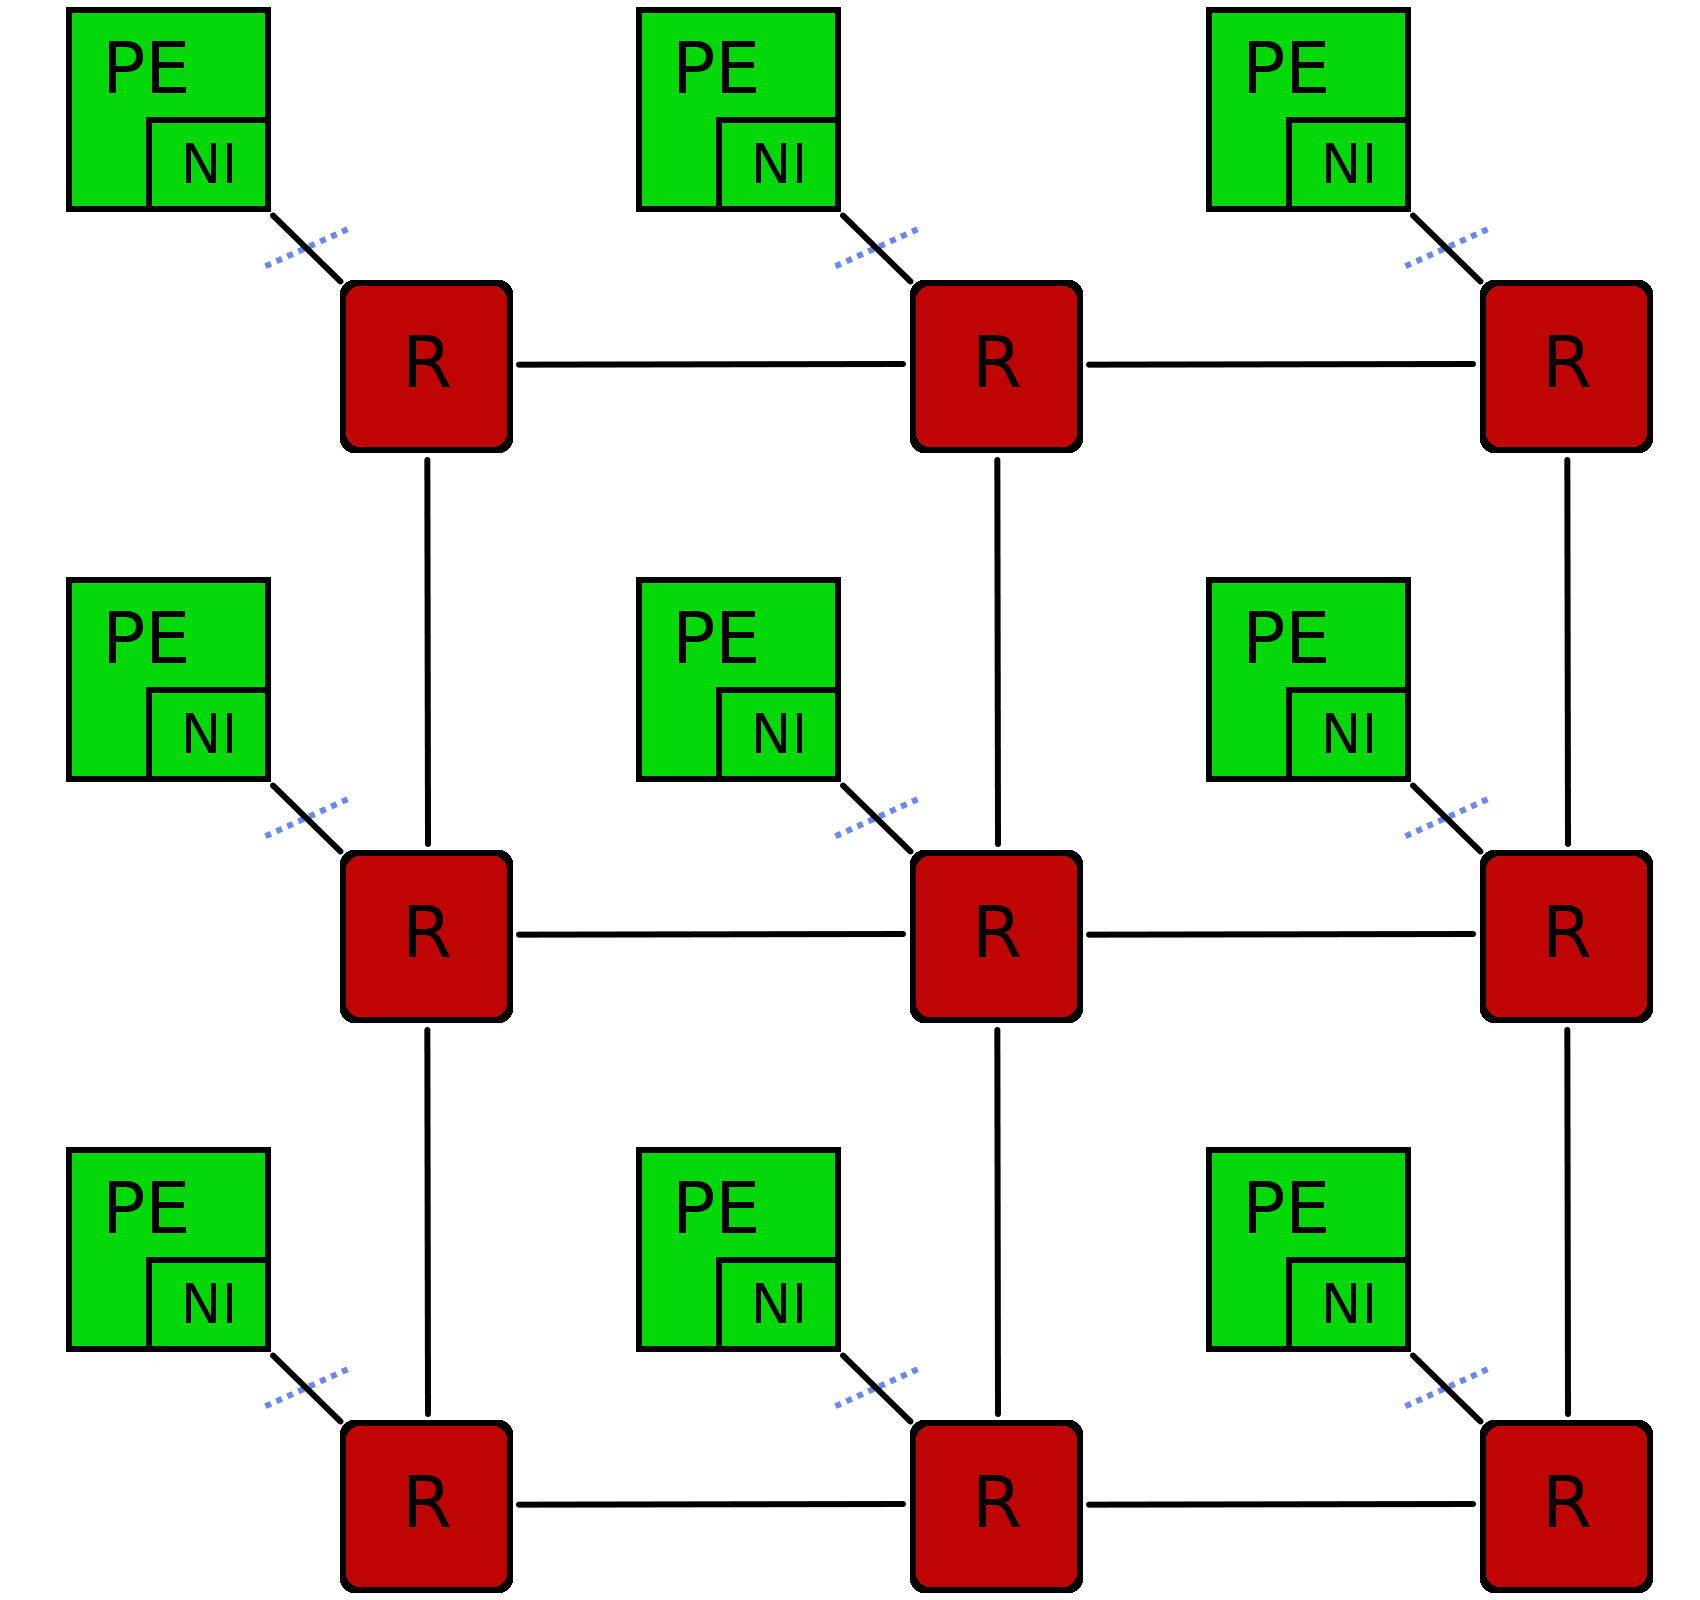
\includegraphics[width=0.6\textwidth]{noc-trust-boundaries}
    \caption[Trust boundaries in a NoC]{Visualization of the trusted and untrusted hardware components in a NoC. The processing elements and network
    interfaces, which are assumed to be trusted, are marked green. The network itself, which is comprised of the routers and their interconnections,
    is not trustworthy and thus marked red. The dotted lines at the local connections mark the trust boundaries.}
    \label{fig:noctrustboundaries}
\end{figure}

\section{Encryption And Authentication}\label{sec:encandauth}
The intent of integrating encryption and authentication is to provide confidentiality and integrity to messages passing through a \gls{noc}. To
implement this, a novel network interface design is proposed. Since all flits that enter the \gls{noc} must pass through a network interface, this is the
ideal location to implement cryptographic protections. In the proposed design, it encrypts all outgoing flits, which can only be decrypted by the
receiver. In addition, a \gls{mac} is computed that is sent together with the encrypted data. On the receiver side, the flits are decrypted and the
\gls{mac} is verified. This scheme is illustrated in Figure \vref{fig:nocflitencauth} and further explained in Section (insert ref here).

\begin{figure}
    \centering
    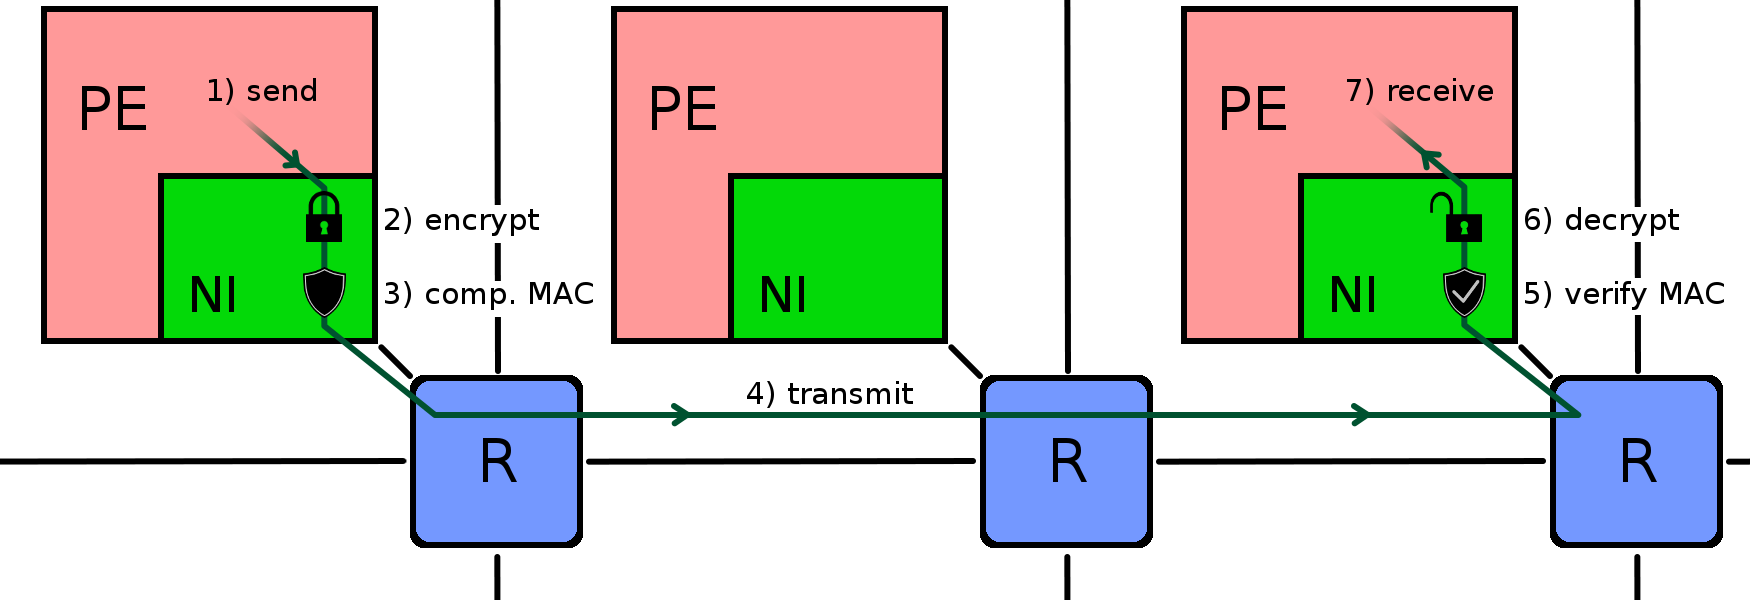
\includegraphics[width=0.9\textwidth]{noc-message-enc-auth}
    \caption[Flit in the NoC with encryption and authentication]{Example of a flit being transmitted through a NoC. After a processing element sends a flit (1),
    encryption is applied (2) and a MAC is computed (3) in the sender's network interface. The encrypted flit and the MAC are then routed to the
    destination (4). There, the receiver's network interface verifies the MAC (5) and decrypts the flit (6). Finally, the flit is passed to the
    receiving processing element (7). This scheme corresponds to the uncoded individual authentication protocol variant.}
    \label{fig:nocflitencauth}
\end{figure}

The constraints imposed by the \gls{noc} environment (cf. Section \ref{sec:networkonchipfun}) make the implementation of security measures a
challenging task. To meet them, only symmetric ciphers were investigated, as they allow for fast computations and low-area implementations.
Furthermore, the produced \glspl{mac} are short enough to fit into a single flit. However, their usage implies that each pair of
sender and receiver needs to possess two shared secret keys (one for encryption and one for authentication). To obtain or renegotiate
such keys in a secure manner, a key exchange algorithm is required
\footnote{One way to realize a secure key exchange in the context of \glspl{noc} is the utilization of central key-keeper cores
\cite{gebotys03securityframework} (see also Section \ref{subsec:securityzones}). Another option is physical layer key generation, as suggested in the
\gls{haec} presentation paper \cite[4]{matthiesen17haec}.}.
As this exceeds the scope of this thesis, each pair of sender and receiver is assumed to have access to the necessary keys. The alternative, asymmetric
cryptography, is not considered since it \enquote{implies a high computational effort} \cite[3]{moriam18activeattackers}. Additionally, this class of
algorithms produces signatures instead of \glspl{mac}, which are \enquote{too long to be included in a flit} \cite[3]{moriam18activeattackers}.

\section{Network Coding}\label{sec:networkcodingover}
A promising approach to improve the performance of \glspl{noc} is network coding. \citeauthor{moriam15manycorenc} have shown that it is particularly
effective in error-prone networks, decreasing latency up to 95\% \cite[7]{moriam15manycorenc}. In the context of this thesis, \glspl{noc} are assumed
to be unreliable: compromised routers may deliberately inject faults or drop flits. Hence, this approach is taken up here to improve the network
performance.

While network coding provides robustness against sporadic flit loss, it does not offer any guarantees on the integrity of flits. Thus, modifications
during the transmission of the coded data are not detected directly, potentially leading to faulty decodings. This deficit is remedied by the cryptographic
layer described above. To evaluate the consequences of the integration of network coding, uncoded versions of the protocol were implemented and
examined as well (see Section \ref{sec:protocolvariants}).

\section{Multipath Routing}
The exploration of different routing strategies is a central aspect of this thesis. Both static and dynamic strategies were
examined and evaluated. With a static strategy, there is a predetermined, time-invariant path that a flit will take to reach a certain destination
from a particular sender. In contrast, dynamic strategies implement random factors that influence the routing decisions for each
transmission. The emphasis of this thesis lies on the latter in order to capture the envisioned benefits of multipath routing.

As a deterministic strategy, dimension order routing is used. On the dynamic side, \gls{dm} and \gls{romm} routing are explored. The properties and
details of these strategies are presented in depth in Section (insert ref here).% TODO: rewrite this a bit, focus on dynamic

\section{Reliability}\label{sec:reliability}
In case the proposed techniques fail to achieve flawless transmission of a flit or generation, it is crucial to provide a method for requesting
their retransmission. This occurs when the integrity check via \gls{mac} verification fails, indicating a modification in one or more of the
associated flits. Furthermore, it is necessary when not enough flits arrive at the destination in time to perform the verifications in the first place.
Additionally, the network coded variants require at least partially intact transmissions in order to successfully decode a generation, necessitating
retransmissions otherwise.

A retransmission scheme is integrated into the protocol by means of \glspl{arq}. If one or more of the aforementioned events occur, the affected
receiver will issue an \gls{arq} back to the sender, who will then resend the flits in question.

To render retransmissions possible, a copy of each flit that is sent through the network must be kept by the sender in order to answer a potential
\gls{arq} arriving later on. This is facilitated by a retransmission buffer that is included in every network interface. Each flit that is sent to the
network (except for the \glspl{arq} themselves) must pass through this buffer, where a copy of it is stored. When an \gls{arq} arrives from another
node, the requested flits are retrieved from the buffer and resent. As the retransmission buffer cannot grow infinitely in size, old flits are
replaced in a \gls{fifo} manner once maximum size is reached.

\section{Protocol Variants}\label{sec:protocolvariants}
To unearth and analyze the most efficient way of applying the ideas outlined above, different variants of the protocol were implemented. They differ
in the way the authentication \glspl{mac} are included in the flit transmissions. Furthermore, both network coded and uncoded versions are compared to
examine the effects of network coding in combination with the cryptographic procedures. The emphasis of this thesis, however, is put on the network
coded forms.

The examined variants are \textit{individual authentication}, \textit{interwoven authentication}, and \textit{full-generation authentication}. For the
first two, both uncoded and network coded variants are implemented. For the latter, only a network coded version is feasible: the authentication
scheme relies on the existance of generations. A comprehensive description of all variants is given in Section
\ref{sec:theprotocol}. % TODO: wiederholung mit "both uncoded and network coded versions/variants"

\section{Analysis And Evaluation}
The aforementioned protocol variants were thoroughly analyzed to empirically determine their quality and suitability for the task at hand. Many
experiments were conducted through software simulation of an \gls{mpsoc} with a \gls{noc} using varying parameters, component layouts, and design
decisions.

The experiments were performed with a simulator specifically crafted for this thesis. Based on the free and open source framework \textit{\omnet{}} \cite{omnet}, it allows
for cycle-accurate simulations with fully customizable statistics recording. Furthermore, its modular design allows for quickly swapping and
reordering components, which is required to test the different protocol variants. The details of the implementation are described in Chapter
\ref{ch:implementation}.

The workflow of the evaluation was as follows: at first, the hyperparameters were determined once, with the resulting values being used in all
subsequent experiments. These hyperparameters include, e.g., the number of required parallel crypto modules\footnote{The term \textit{crypto modules} is
used to refer to both encryption and authentication modules.} per network interface and the \gls{arq} timeouts. Afterwards, the remaining parameters are
varied to find the optimal configuration for each protocol variant. Finally, the most promising of these variants is identified. The full evaluation
process is elaborated in Chapter \ref{ch:evaluation}.
